\section{CAPÍTULO V: Producto final}

Este capítulo presenta la documentación completa del producto final, incluyendo los manuales necesarios para que usuarios finales y personal técnico puedan utilizar, operar y mantener la plataforma educativa 3D de gamificación de tareas académicas. Se incluyen dos manuales fundamentales: el Manual del Usuario, orientado a estudiantes, docentes y administradores que interactuarán con la plataforma; y el Manual del Sistema, dirigido al personal técnico encargado de la instalación, configuración, mantenimiento y resolución de problemas del sistema.

\subsection{5.1 Manual de usuario}

El Manual del Usuario proporciona instrucciones detalladas sobre el uso de la plataforma desde la perspectiva de los tres roles principales: estudiantes, docentes y administradores. Cada sección incluye guías paso a paso, capturas de pantalla y buenas prácticas para maximizar el valor educativo de la aplicación.

\subsubsection{5.1.1 Introducción a la plataforma}

La plataforma Warclass es una aplicación educativa 3D que transforma las tareas académicas tradicionales en experiencias de aprendizaje inmersivas mediante la gamificación. El sistema permite a los docentes crear misiones educativas que los estudiantes completan en un entorno virtual medieval, ganando puntos, subiendo de nivel y desbloqueando logros mientras aprenden.

\paragraph{Acceso a la plataforma}

La plataforma está disponible en versión web y móvil:

\begin{itemize}
	\item \textbf{Versión Web}: Accesible desde cualquier navegador moderno (Chrome, Firefox, Safari, Edge) en la URL proporcionada por su institución educativa.
	\item \textbf{Versión Móvil}: Aplicación nativa disponible para Android e iOS, descargable desde las tiendas oficiales.
\end{itemize}

\paragraph{Requisitos del sistema}

\begin{table}[H]
	\centering
	\caption{Requisitos mínimos del sistema para usuarios.}
	\begin{tabular}{p{4cm} p{9cm}}
		\toprule
		Componente & Requisitos \\
		\midrule
		Navegador Web & Chrome 90+, Firefox 88+, Safari 14+, Edge 90+ \\
		Conexión Internet & Mínimo 5 Mbps (10 Mbps recomendado) \\
		Resolución & 1366x768 mínimo (1920x1080 recomendado) \\
		Hardware & CPU: Dual Core 2.0 GHz, RAM: 4GB, GPU: Compatible WebGL 2.0 \\
		Sistema Operativo Móvil & Android 9.0+ o iOS 13.0+ \\
		\bottomrule
	\end{tabular}
\end{table}

\subsubsection{5.1.2 Registro y autenticación}

\paragraph{Crear una cuenta}

Los usuarios pueden registrarse utilizando su correo institucional o mediante autenticación OAuth2 con proveedores autorizados (Google Workspace, Microsoft 365).

\textbf{Proceso de registro con correo institucional:}

\begin{enumerate}
	\item Acceder a la URL de la plataforma proporcionada por su institución
	\item Hacer clic en el botón ``Registrarse''
	\item Ingresar correo electrónico institucional
	\item Crear una contraseña segura (mínimo 8 caracteres, incluyendo mayúsculas, minúsculas, números y símbolos)
	\item Completar datos del perfil: nombre completo, código de estudiante/docente, institución
	\item Aceptar los términos de servicio y políticas de privacidad
	\item Verificar el correo electrónico mediante el enlace enviado
	\item Iniciar sesión con las credenciales creadas
\end{enumerate}

\begin{figure}[H]
	\centering
	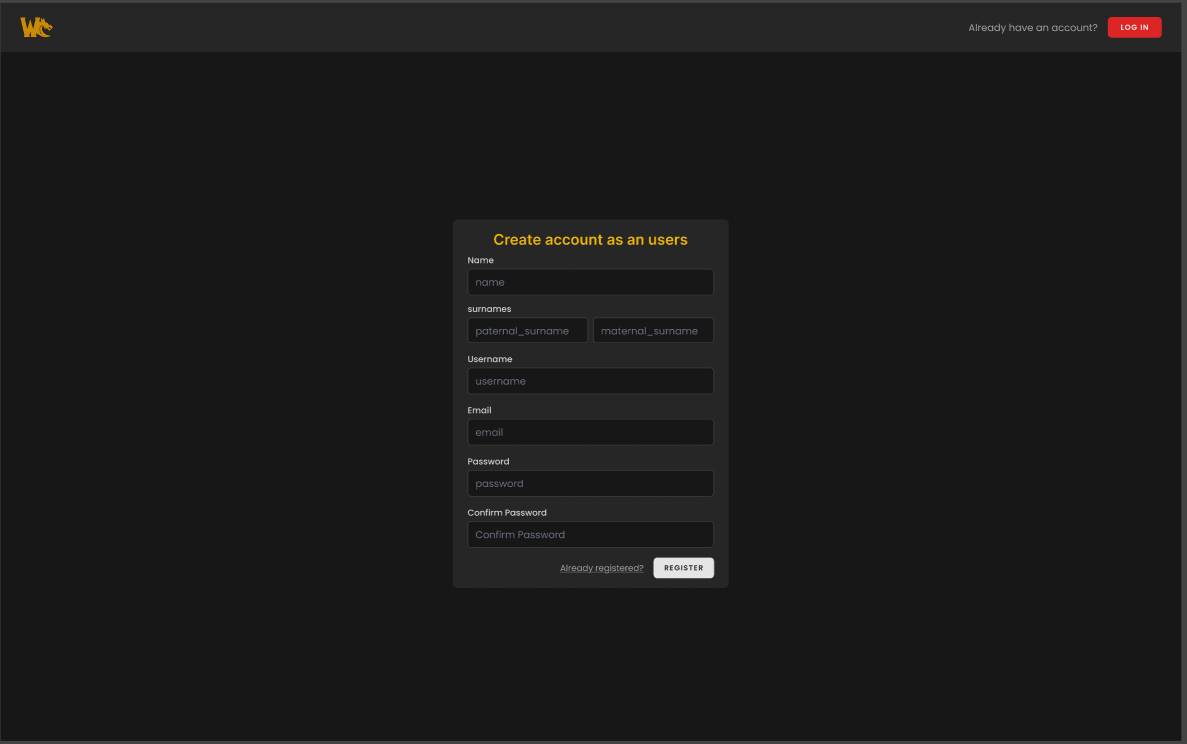
\includegraphics[width=0.75\textwidth]{images/pagina_web_registro.png}
	\caption{Pantalla de registro de usuario con formulario de datos básicos.}
	\label{fig:manual-registro}
\end{figure}

\textbf{Proceso de registro con OAuth2:}

\begin{enumerate}
	\item Hacer clic en ``Iniciar sesión con Google'' o ``Iniciar sesión con Microsoft''
	\item Autorizar el acceso a su cuenta institucional
	\item Completar datos adicionales si es necesario
	\item Confirmar creación de cuenta
\end{enumerate}

\begin{figure}[H]
	\centering
	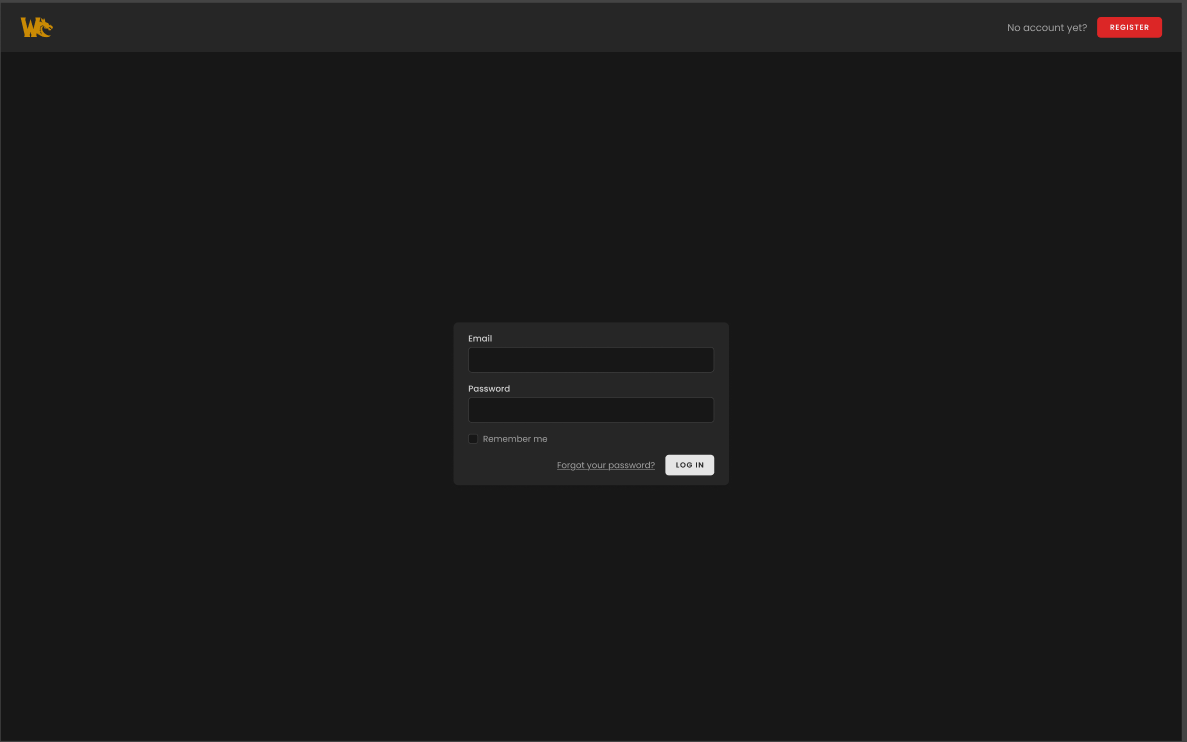
\includegraphics[width=0.75\textwidth]{images/pagina_web_iniciar-sesion.png}
	\caption{Pantalla de inicio de sesión con opciones de autenticación.}
	\label{fig:manual-login}
\end{figure}

\paragraph{Inicio de sesión}

\begin{enumerate}
	\item Ingresar correo electrónico y contraseña
	\item (Opcional) Marcar ``Recordarme'' para mantener la sesión activa
	\item Hacer clic en ``Iniciar sesión''
	\item Si olvidó su contraseña, usar la opción ``¿Olvidaste tu contraseña?''
\end{enumerate}

\paragraph{Recuperación de contraseña}

\begin{enumerate}
	\item Hacer clic en ``¿Olvidaste tu contraseña?''
	\item Ingresar correo electrónico registrado
	\item Revisar bandeja de entrada y seguir las instrucciones del correo
	\item Crear nueva contraseña segura
	\item Iniciar sesión con la nueva contraseña
\end{enumerate}

\subsubsection{5.1.3 Manual para estudiantes}

\paragraph{Dashboard del estudiante}

Al iniciar sesión, el estudiante accede a su dashboard personalizado que muestra:

\begin{itemize}
	\item \textbf{Vista del avatar 3D}: Representación visual del progreso y equipamiento actual
	\item \textbf{Nivel y experiencia (XP)}: Barra de progreso que muestra el nivel actual y experiencia necesaria para el siguiente nivel
	\item \textbf{Misiones activas}: Lista de tareas académicas disponibles y en progreso
	\item \textbf{Notificaciones}: Alertas de nuevas misiones, logros desbloqueados y mensajes de docentes
	\item \textbf{Logros recientes}: Insignias y reconocimientos obtenidos
	\item \textbf{Estadísticas}: Tiempo de estudio, misiones completadas, puntos ganados
\end{itemize}

\paragraph{Personalización del avatar}

El avatar 3D es la representación visual del estudiante en el entorno virtual. Su apariencia evoluciona con el progreso académico.

\textbf{Pasos para personalizar el avatar:}

\begin{enumerate}
	\item Hacer clic en el avatar en el dashboard
	\item Seleccionar la pestaña ``Personalizar''
	\item Elegir características disponibles según el nivel:
	\begin{itemize}
		\item \textbf{Género}: Masculino, Femenino, Otro
		\item \textbf{Tono de piel}: Paleta de colores disponible
		\item \textbf{Cabello}: Estilo y color (se desbloquean con niveles)
		\item \textbf{Ojos}: Color y forma
		\item \textbf{Ropa}: Atuendos medievales desbloqueables
		\item \textbf{Accesorios}: Armas decorativas, escudos, capas (requieren logros)
	\end{itemize}
	\item Previsualizar cambios en tiempo real en el visor 3D
	\item Hacer clic en ``Guardar cambios''
\end{enumerate}

\paragraph{Explorar y aceptar misiones}

Las misiones son las actividades académicas gamificadas creadas por los docentes.

\textbf{Tipos de misiones:}

\begin{itemize}
	\item \textbf{Misión Principal}: Actividad obligatoria vinculada al currículo
	\item \textbf{Misión Secundaria}: Actividad opcional para refuerzo o profundización
	\item \textbf{Misión de Grupo}: Actividad colaborativa con otros estudiantes
	\item \textbf{Desafío}: Competencia temporal con recompensas especiales
\end{itemize}

\textbf{Aceptar una misión:}

\begin{enumerate}
	\item Navegar a la sección ``Misiones Disponibles''
	\item Hacer clic en una misión para ver los detalles:
	\begin{itemize}
		\item Descripción y objetivos de aprendizaje
		\item Dificultad (Novato, Aprendiz, Experto, Maestro)
		\item Recompensas (XP, puntos, ítems)
		\item Fecha límite
		\item Materiales de apoyo
	\end{itemize}
	\item Hacer clic en ``Aceptar Misión''
	\item La misión aparecerá en ``Mis Misiones Activas''
\end{enumerate}

\paragraph{Completar misiones}

\textbf{Desarrollo de la misión:}

\begin{enumerate}
	\item Acceder a la misión desde ``Mis Misiones Activas''
	\item Leer las instrucciones y objetivos específicos
	\item Acceder a materiales de apoyo (videos, documentos, enlaces)
	\item Completar las actividades requeridas:
	\begin{itemize}
		\item Responder cuestionarios interactivos
		\item Subir archivos de trabajo (documentos, imágenes, videos)
		\item Participar en debates en el foro de la misión
		\item Realizar investigaciones y análisis
	\end{itemize}
	\item Usar el chatbot de ayuda si tiene dudas
	\item Guardar progreso automático (la plataforma guarda cada 30 segundos)
	\item Cuando termine, hacer clic en ``Enviar Misión''
\end{enumerate}

\textbf{Evaluación y retroalimentación:}

\begin{enumerate}
	\item El sistema evalúa automáticamente componentes objetivos (cuestionarios, ejercicios)
	\item El docente revisa componentes subjetivos (ensayos, proyectos)
	\item Recibe notificación cuando la misión sea evaluada
	\item Puede ver:
	\begin{itemize}
		\item Calificación obtenida
		\item Comentarios del docente
		\item Áreas de mejora
		\item Respuestas correctas e incorrectas
	\end{itemize}
	\item Si es posible, puede reenviar la misión para mejorar la calificación
\end{enumerate}

\paragraph{Sistema de progresión}

\textbf{Niveles y experiencia (XP):}

\begin{itemize}
	\item Cada misión completada otorga XP según su dificultad
	\item Al acumular suficiente XP, el estudiante sube de nivel
	\item Cada nivel desbloquea nuevas personalizaciones para el avatar
	\item Los niveles se muestran como rangos medievales: Paje (1-5), Escudero (6-10), Caballero (11-20), Paladín (21-30), Leyenda (31+)
\end{itemize}

\textbf{Sistema de puntos:}

\begin{itemize}
	\item Puntos de Conocimiento: Reflejan el dominio académico
	\item Puntos de Participación: Recompensan el engagement
	\item Puntos de Colaboración: Otorgados en misiones grupales
\end{itemize}

\textbf{Logros e insignias:}

\begin{itemize}
	\item \textbf{Logros de dominio}: Por completar conjuntos de misiones relacionadas
	\item \textbf{Logros de velocidad}: Por completar misiones antes del plazo
	\item \textbf{Logros de excelencia}: Por obtener calificaciones perfectas
	\item \textbf{Logros sociales}: Por colaborar efectivamente
	\item \textbf{Logros especiales}: Eventos temporales y desafíos únicos
\end{itemize}

\paragraph{Tabla de clasificación}

La tabla muestra el ranking de estudiantes según diversos criterios:

\begin{itemize}
	\item Ranking general por XP total
	\item Ranking por curso específico
	\item Ranking semanal/mensual
	\item Comparación con compañeros de grupo
\end{itemize}

\textbf{Nota sobre privacidad:} Los estudiantes pueden optar por aparecer de forma anónima en las tablas públicas.

\subsubsection{5.1.4 Manual para docentes}

\paragraph{Dashboard del docente}

El panel de control del docente proporciona una vista integral de todas sus actividades educativas:

\begin{itemize}
	\item \textbf{Resumen de cursos}: Lista de cursos activos con métricas rápidas
	\item \textbf{Misiones pendientes de evaluación}: Trabajos esperando revisión
	\item \textbf{Estadísticas de engagement}: Participación estudiantil en tiempo real
	\item \textbf{Alertas}: Estudiantes con bajo rendimiento o inactividad
	\item \textbf{Analítica}: Gráficos de progreso del grupo
\end{itemize}

\begin{figure}[H]
	\centering
	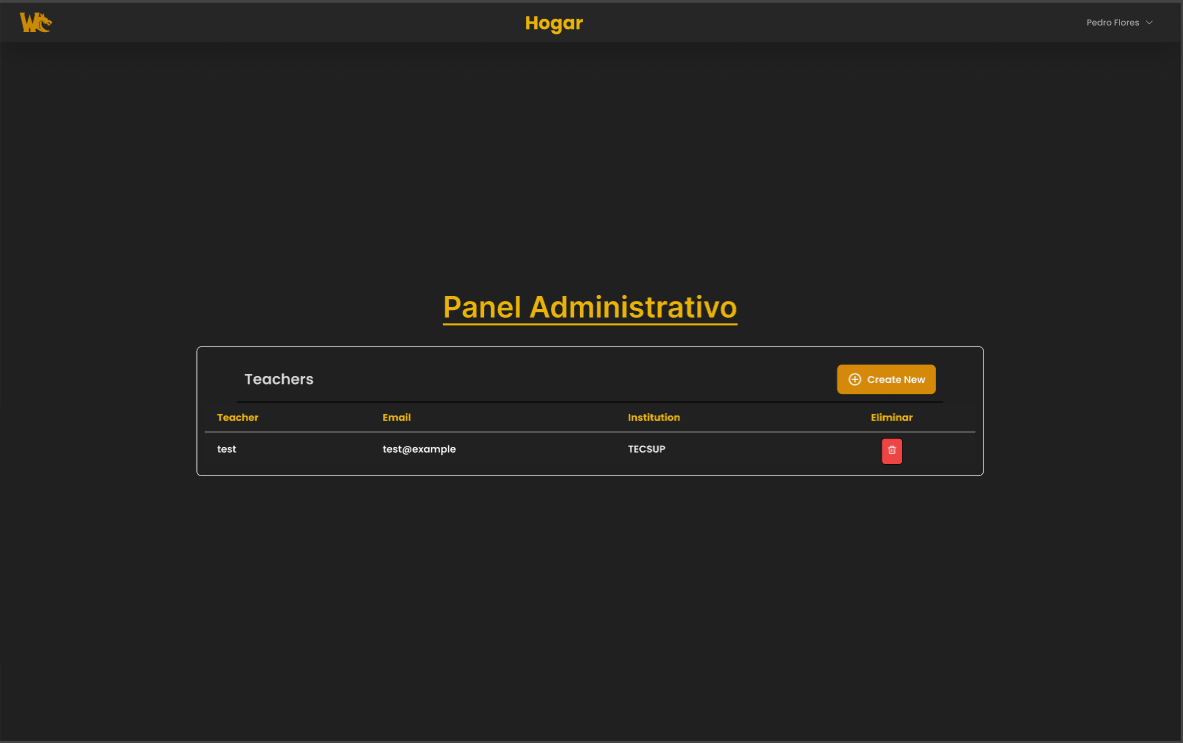
\includegraphics[width=0.75\textwidth]{images/pagina_web_panel-administrativo.png}
	\caption{Panel de administración del docente con vista de cursos y misiones activas.}
	\label{fig:manual-profesor}
\end{figure}

\paragraph{Gestión de cursos}

\textbf{Crear un nuevo curso:}

\begin{enumerate}
	\item Ir a ``Mis Cursos'' > ``Crear Nuevo Curso''
	\item Completar información básica:
	\begin{itemize}
		\item Nombre del curso
		\item Código de curso
		\item Descripción y objetivos de aprendizaje
		\item Período académico
		\item Horario y modalidad
	\end{itemize}
	\item Configurar ajustes de gamificación:
	\begin{itemize}
		\item Esquema de puntos (XP por dificultad)
		\item Niveles y rangos personalizados
		\item Logros específicos del curso
	\end{itemize}
	\item Establecer políticas:
	\begin{itemize}
		\item Política de entregas tardías
		\item Número de reenvíos permitidos
		\item Criterios de evaluación
	\end{itemize}
	\item Hacer clic en ``Crear Curso''
\end{enumerate}

\begin{figure}[H]
	\centering
	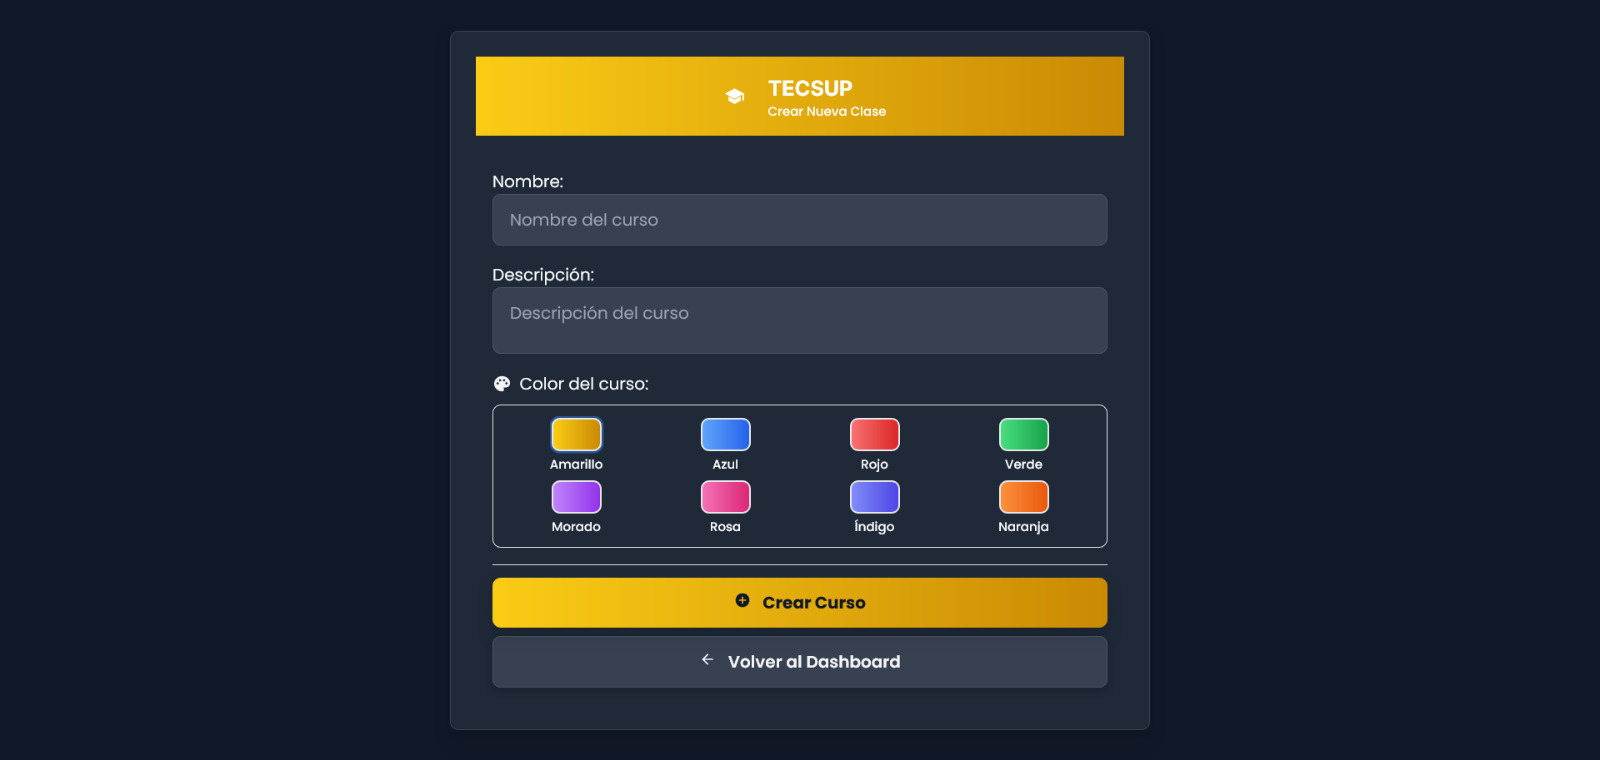
\includegraphics[width=0.75\textwidth]{images/pagina_web_crear-una-clase.jpg}
	\caption{Interfaz para crear un nuevo curso con configuración básica.}
	\label{fig:manual-crear-curso}
\end{figure}

\begin{figure}[H]
	\centering
	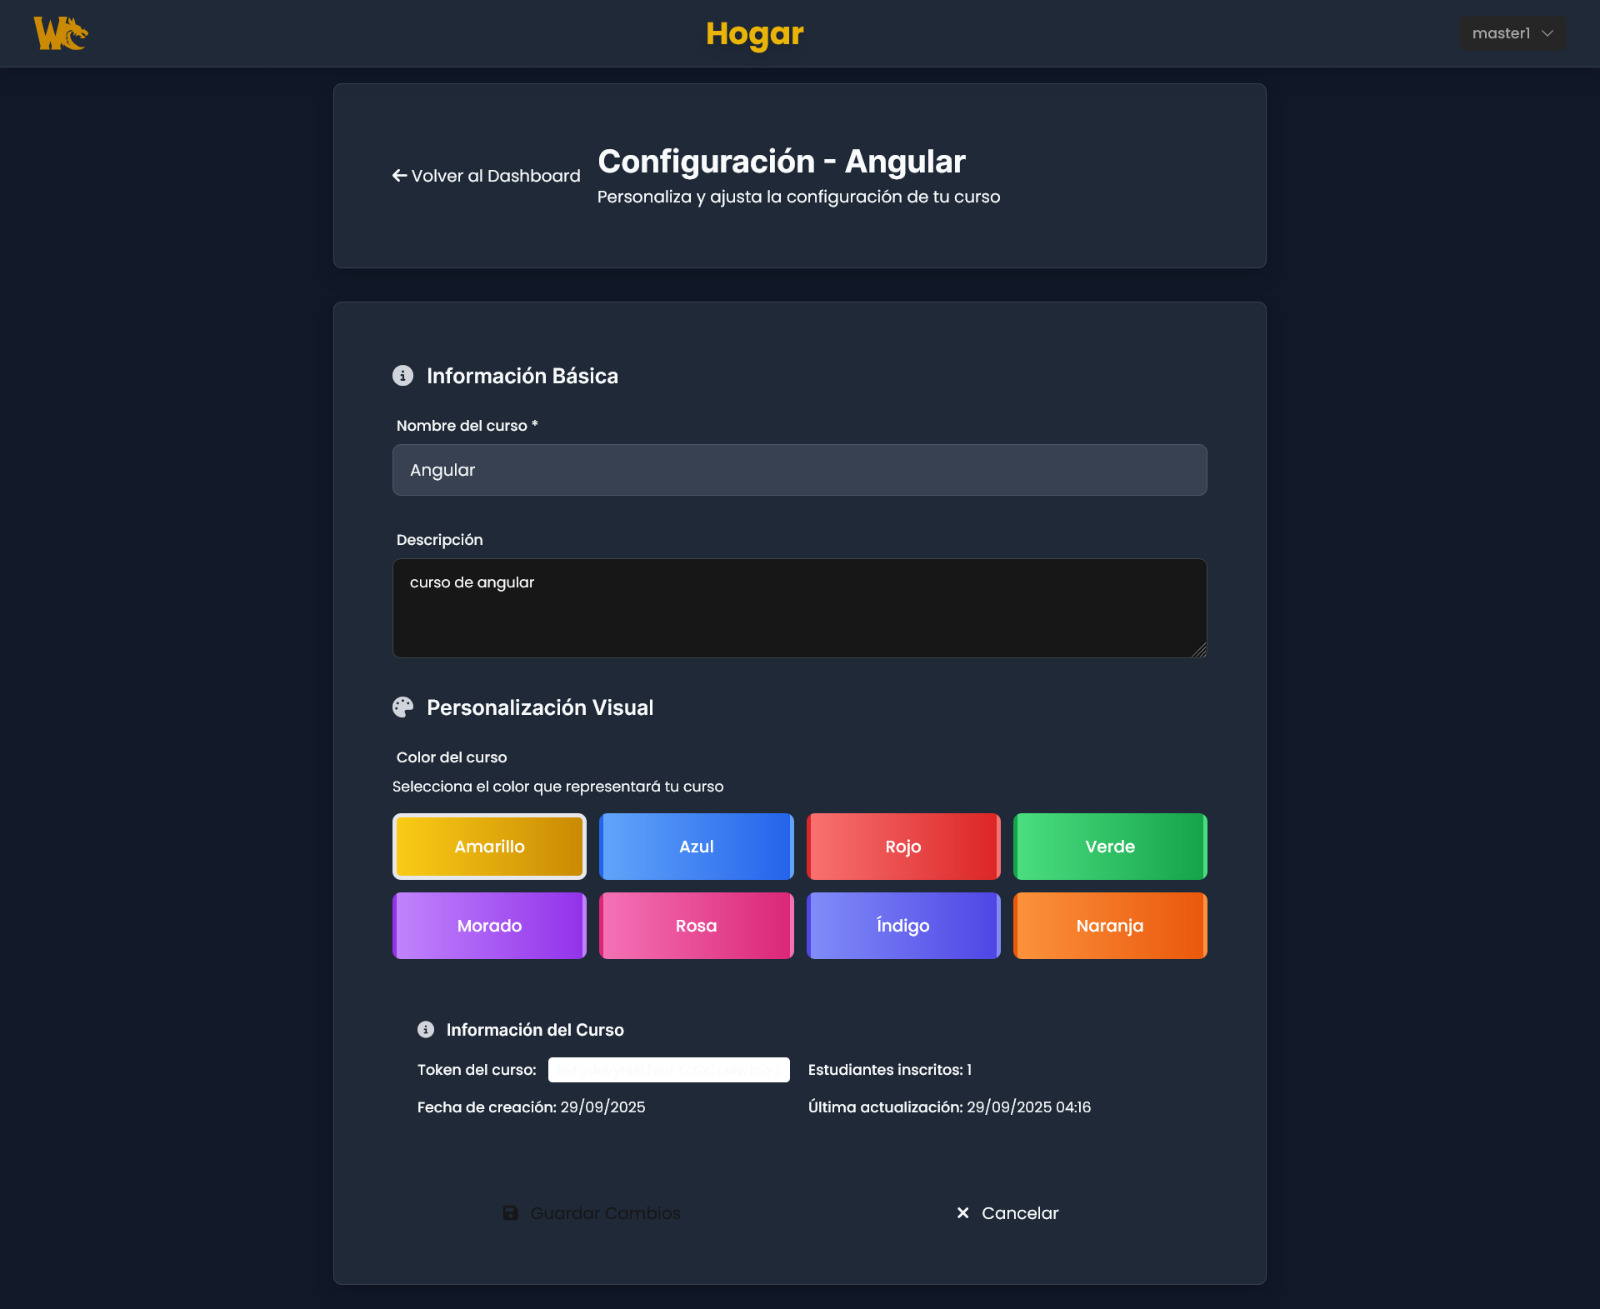
\includegraphics[width=0.75\textwidth]{images/pagina_web_configuracion-de-la.clase.jpg}
	\caption{Configuración de ajustes de gamificación y políticas del curso.}
	\label{fig:manual-config-curso}
\end{figure}

\begin{figure}[H]
	\centering
	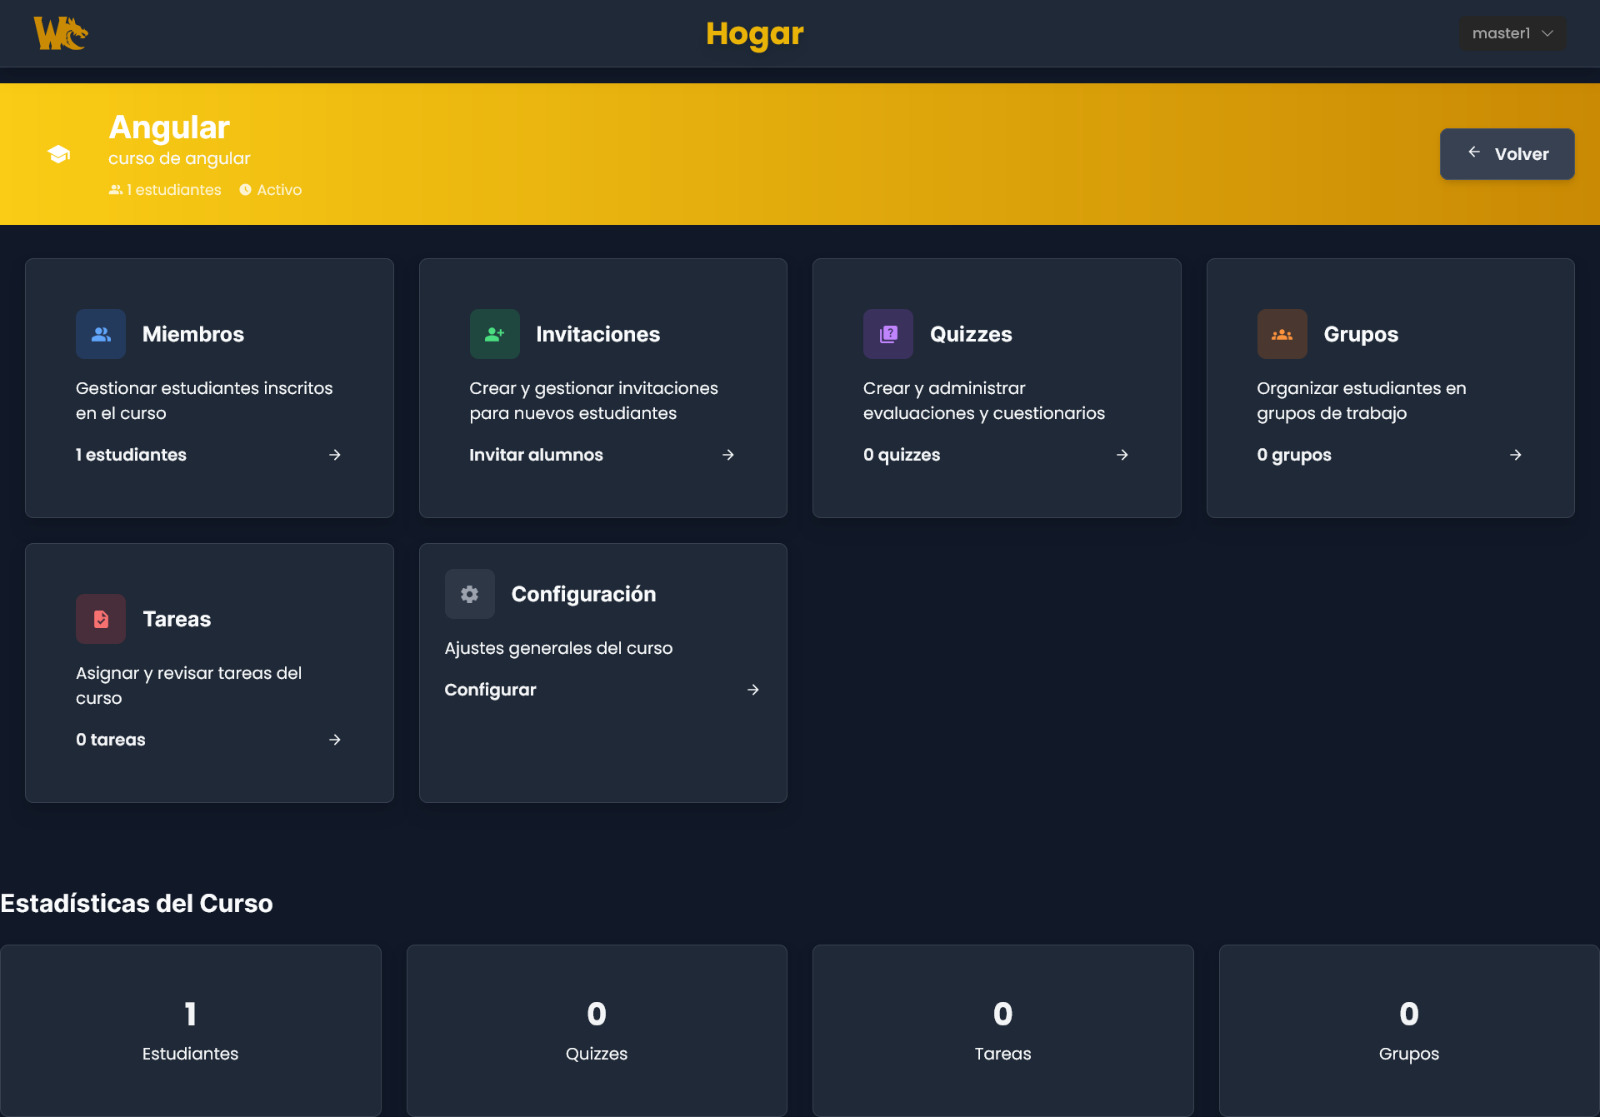
\includegraphics[width=0.75\textwidth]{images/pagina_web_vista-profesor-clase.jpg}
	\caption{Vista principal del profesor para gestión del curso.}
	\label{fig:manual-vista-profesor}
\end{figure}

\textbf{Gestionar estudiantes:}

\begin{enumerate}
	\item Acceder al curso > ``Estudiantes''
	\item Opciones disponibles:
	\begin{itemize}
		\item \textbf{Agregar estudiantes}: Mediante código de curso, lista de correos o integración con Canvas
		\item \textbf{Organizar grupos}: Crear equipos para misiones colaborativas
		\item \textbf{Ver perfiles}: Revisar progreso individual, historial y logros
		\item \textbf{Enviar mensajes}: Comunicación directa o masiva
		\item \textbf{Gestionar permisos}: Roles especiales (moderador de foro, tutor par)
	\end{itemize}
\end{enumerate}

\begin{figure}[H]
	\centering
	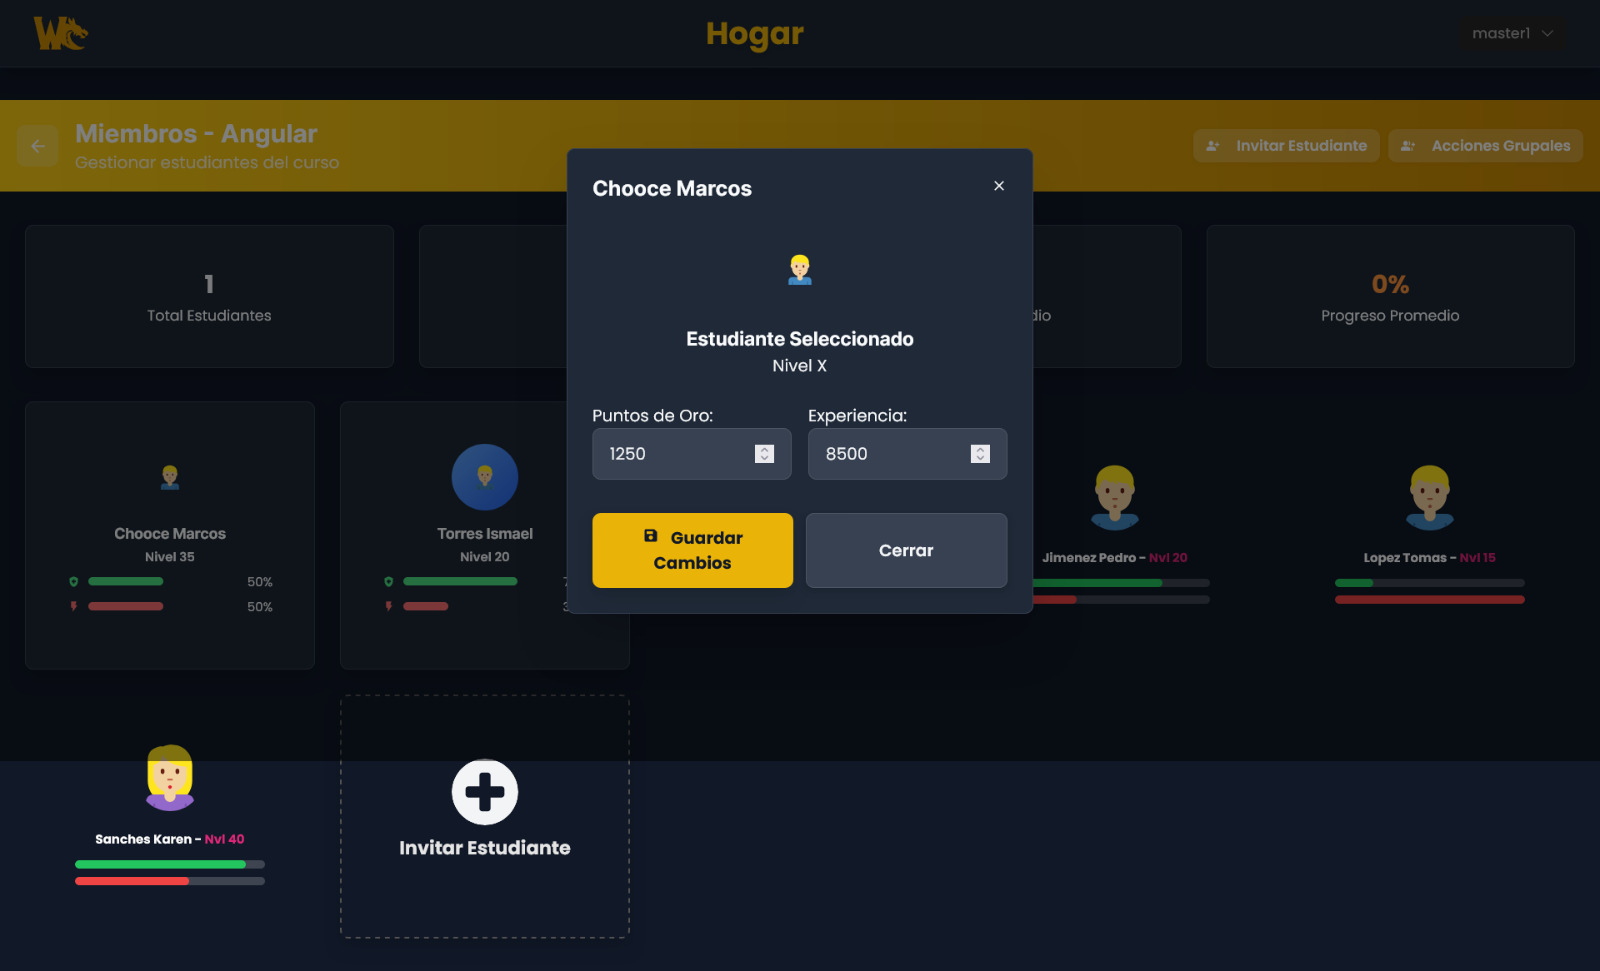
\includegraphics[width=0.75\textwidth]{images/pagina_web_gestionar-alumnos.jpg}
	\caption{Interfaz de gestión de estudiantes con opciones de organización y permisos.}
	\label{fig:manual-gestionar-alumnos}
\end{figure}

\begin{figure}[H]
	\centering
	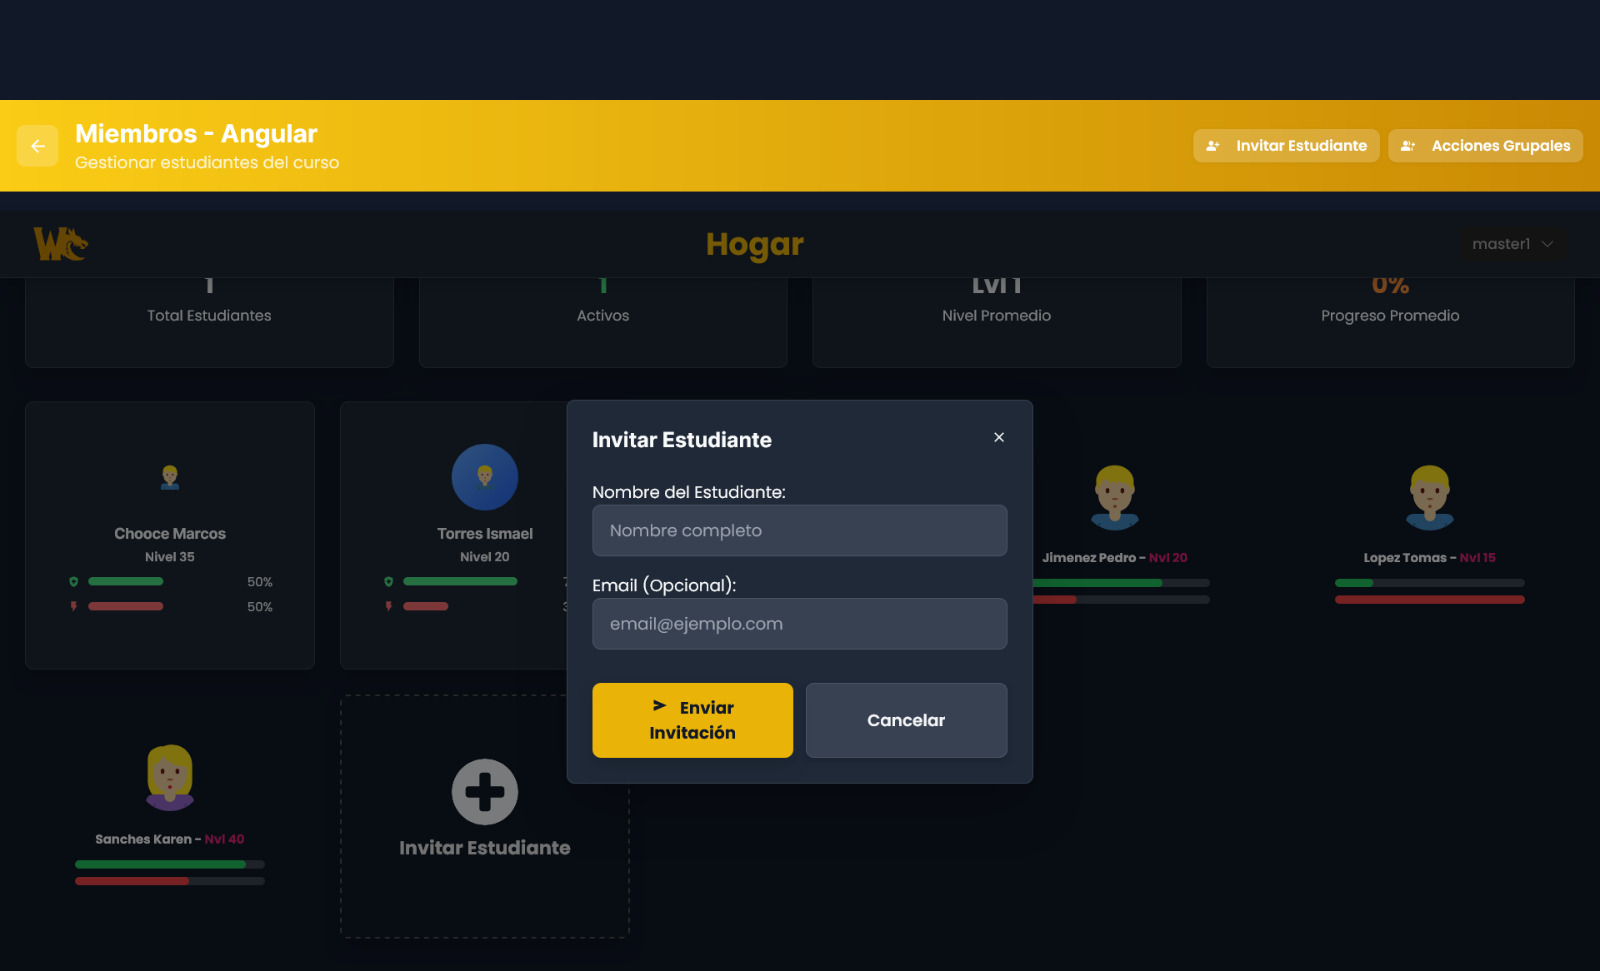
\includegraphics[width=0.75\textwidth]{images/pagina_web_invitar-a-clase.jpg}
	\caption{Sistema de invitación de estudiantes mediante código o correo electrónico.}
	\label{fig:manual-invitar-clase}
\end{figure}

\begin{figure}[H]
	\centering
	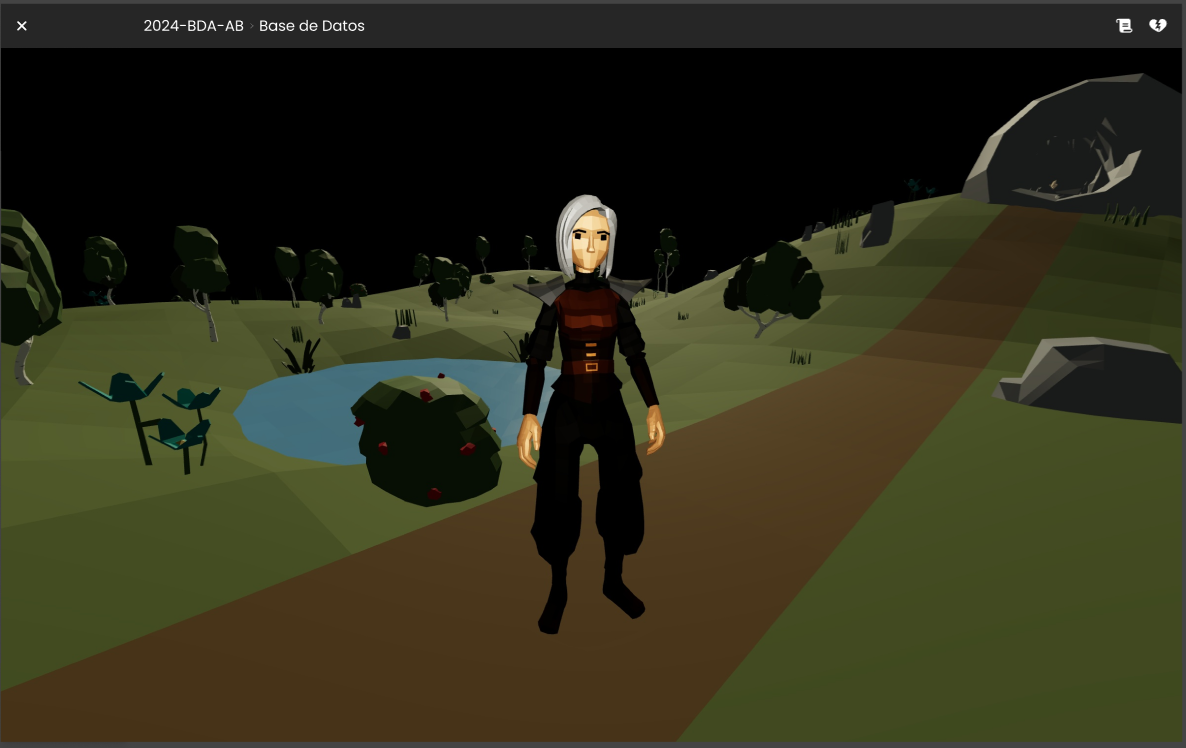
\includegraphics[width=0.75\textwidth]{images/pagina_web_vista-alumno.png}
	\caption{Vista del estudiante mostrando su avatar y progreso en el sistema.}
	\label{fig:manual-vista-alumno}
\end{figure}

\paragraph{Crear misiones educativas}

El creador de misiones permite transformar cualquier actividad académica en una experiencia gamificada.

\textbf{Proceso de creación:}

\begin{enumerate}
	\item Acceder al curso > ``Crear Nueva Misión''
	\item \textbf{Paso 1 - Información básica}:
	\begin{itemize}
		\item Título de la misión (debe ser atractivo)
		\item Descripción narrativa (contextualizar en el mundo medieval)
		\item Tipo de misión (Principal, Secundaria, Grupal, Desafío)
		\item Curso y tema asociado
	\end{itemize}
	\item \textbf{Paso 2 - Objetivos de aprendizaje}:
	\begin{itemize}
		\item Definir competencias a desarrollar
		\item Indicadores de logro
		\item Nivel de dificultad (Novato, Aprendiz, Experto, Maestro)
	\end{itemize}
	\item \textbf{Paso 3 - Contenido y actividades}:
	\begin{itemize}
		\item Agregar instrucciones detalladas
		\item Subir materiales de apoyo (PDF, videos, enlaces)
		\item Configurar actividades:
		\begin{itemize}
			\item Cuestionarios (opción múltiple, verdadero/falso, respuesta corta)
			\item Tareas de entrega (documentos, imágenes, videos)
			\item Foros de discusión
			\item Ejercicios interactivos
		\end{itemize}
	\end{itemize}
	\item \textbf{Paso 4 - Evaluación}:
	\begin{itemize}
		\item Definir criterios de evaluación (rúbricas)
		\item Asignar puntos a cada componente
		\item Configurar evaluación automática para elementos objetivos
		\item Establecer peso de componentes subjetivos
	\end{itemize}
	\item \textbf{Paso 5 - Gamificación}:
	\begin{itemize}
		\item Asignar XP según dificultad
		\item Definir recompensas (ítems virtuales, insignias)
		\item Configurar bonificaciones (por velocidad, calidad)
		\item Agregar logros especiales
	\end{itemize}
	\item \textbf{Paso 6 - Configuración temporal}:
	\begin{itemize}
		\item Fecha de publicación
		\item Fecha límite de entrega
		\item Permitir entregas tardías (con penalización)
		\item Número de intentos permitidos
	\end{itemize}
	\item Previsualizar la misión
	\item Publicar o guardar como borrador
\end{enumerate}

\paragraph{Evaluar trabajos de estudiantes}

\textbf{Proceso de evaluación:}

\begin{enumerate}
	\item Acceder a ``Misiones Pendientes de Evaluación''
	\item Seleccionar una misión para ver las entregas
	\item Para cada estudiante:
	\begin{itemize}
		\item Revisar el trabajo entregado
		\item Ver evaluación automática (si aplica)
		\item Aplicar rúbrica de evaluación
		\item Asignar calificación numérica
		\item Escribir retroalimentación constructiva
		\item Identificar fortalezas y áreas de mejora
		\item Permitir reenvío (opcional)
	\end{itemize}
	\item Guardar evaluación y notificar al estudiante
\end{enumerate}

\begin{figure}[H]
	\centering
	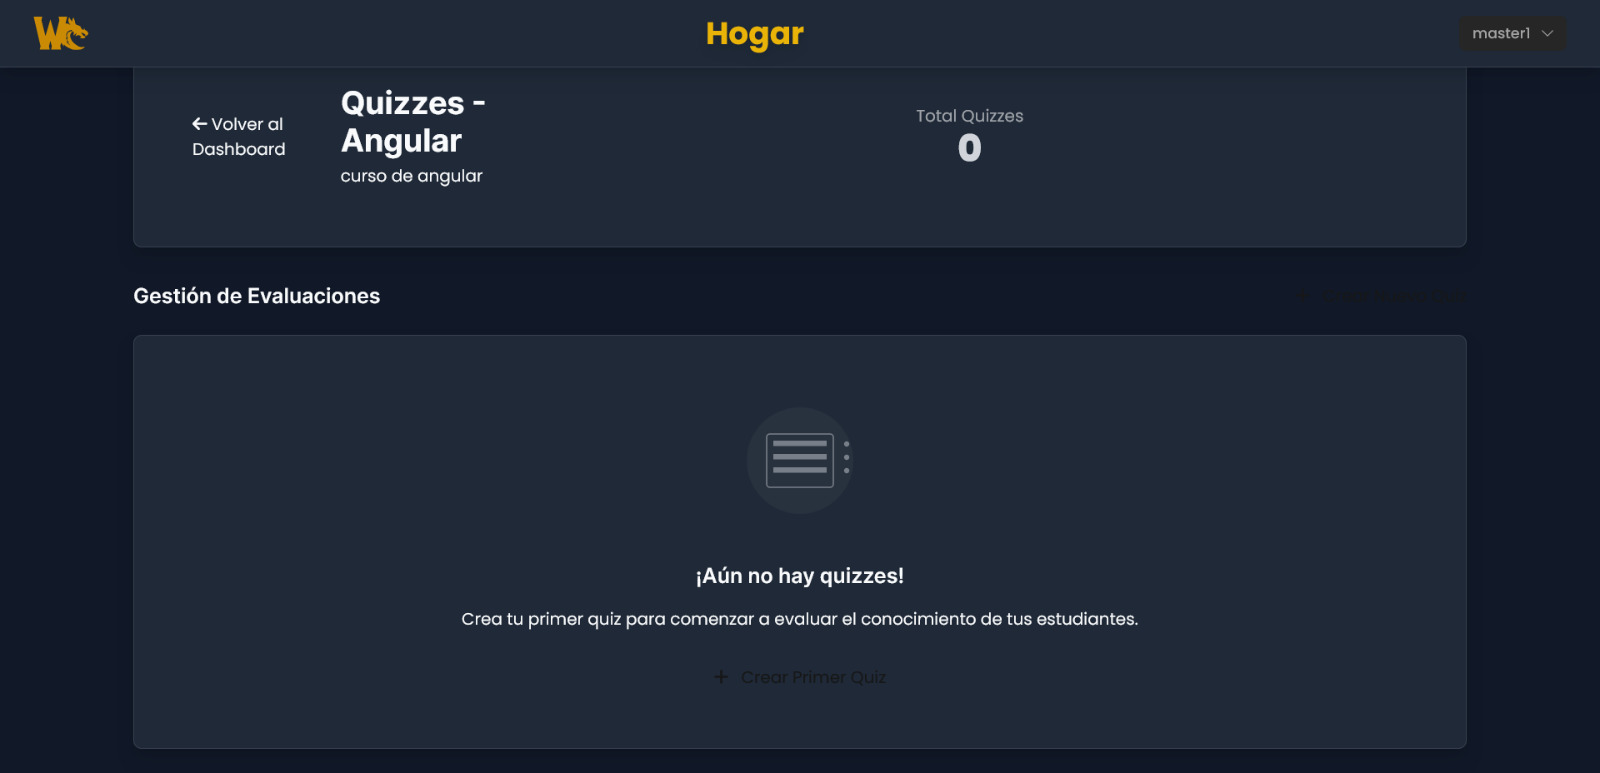
\includegraphics[width=0.75\textwidth]{images/pagina_web_gestion-de-evaluaciones.jpg}
	\caption{Sistema de evaluación y calificación de trabajos de estudiantes.}
	\label{fig:manual-evaluaciones}
\end{figure}

\paragraph{Analítica y seguimiento}

El sistema proporciona herramientas de analítica para monitorear el progreso:

\begin{itemize}
	\item \textbf{Panel de curso}: Métricas generales de participación y rendimiento
	\item \textbf{Gráficos de progreso}: Visualización temporal del avance del grupo
	\item \textbf{Análisis comparativo}: Identificación de misiones con mayor dificultad
	\item \textbf{Alertas tempranas}: Estudiantes en riesgo de abandono o bajo rendimiento
	\item \textbf{Reportes exportables}: Datos en formato CSV/PDF para análisis externo
\end{itemize}

\subsubsection{5.1.5 Manual para administradores}

\paragraph{Dashboard del administrador}

Los administradores institucionales tienen acceso a funcionalidades de gestión global:

\begin{itemize}
	\item \textbf{Gestión de usuarios}: Crear, editar y desactivar cuentas
	\item \textbf{Gestión de instituciones}: Configurar datos institucionales
	\item \textbf{Supervisión de cursos}: Vista global de todos los cursos activos
	\item \textbf{Reportes institucionales}: Métricas de uso y adopción
	\item \textbf{Configuración del sistema}: Parámetros globales de la plataforma
	\item \textbf{Auditoría}: Registro de actividades y eventos del sistema
\end{itemize}

\paragraph{Gestión de usuarios}

\textbf{Crear cuentas masivamente:}

\begin{enumerate}
	\item Ir a ``Administración'' > ``Usuarios'' > ``Importar''
	\item Descargar plantilla CSV
	\item Completar datos: email, nombre, rol, código institucional
	\item Subir archivo CSV
	\item Revisar y confirmar importación
	\item El sistema envía correos de activación automáticamente
\end{enumerate}

\textbf{Gestionar roles y permisos:}

\begin{itemize}
	\item \textbf{Superadministrador}: Control total del sistema
	\item \textbf{Administrador institucional}: Gestión de su institución
	\item \textbf{Coordinador académico}: Supervisión de departamentos
	\item \textbf{Docente}: Creación y gestión de cursos
	\item \textbf{Estudiante}: Participación en cursos
\end{itemize}

\paragraph{Configuración institucional}

\begin{enumerate}
	\item Acceder a ``Configuración'' > ``Institución''
	\item Configurar:
	\begin{itemize}
		\item Datos de la institución (nombre, logo, colores)
		\item Políticas de privacidad y términos de servicio
		\item Proveedores OAuth2 autorizados
		\item Dominios de correo institucional permitidos
		\item Integraciones con LMS (Canvas, Moodle)
		\item Configuración de Discord
	\end{itemize}
	\item Guardar cambios
\end{enumerate}

\paragraph{Monitoreo y reportes}

\begin{itemize}
	\item \textbf{Dashboard ejecutivo}: KPIs de adopción y uso
	\item \textbf{Reportes de engagement}: Tasas de participación por departamento
	\item \textbf{Análisis de rendimiento}: Métricas académicas agregadas
	\item \textbf{Auditoría de sistema}: Eventos de seguridad y accesos
	\item \textbf{Uso de recursos}: Consumo de almacenamiento y ancho de banda
\end{itemize}

\subsection{5.2 Manual del sistema}

El Manual del Sistema proporciona documentación técnica completa para el personal de TI encargado de instalar, configurar, mantener y resolver problemas de la plataforma. Incluye arquitectura del sistema, procedimientos de despliegue, configuración de servicios y guías de troubleshooting.

\subsubsection{5.2.1 Arquitectura del sistema}

\paragraph{Stack tecnológico}

\begin{table}[H]
	\centering
	\caption{Componentes tecnológicos del sistema.}
	\begin{tabular}{p{4cm} p{9cm}}
		\toprule
		Componente & Tecnología \\
		\midrule
		Frontend Web & Next.js 15.5.4, React 18, TypeScript 5 \\
		Entorno 3D & Three.js R150+, WebGL 2.0 \\
		Frontend Móvil & React Native (Expo) \\
		Backend API & Next.js API Routes (TypeScript) \\
		Base de Datos & PostgreSQL 15+ \\
		ORM & Prisma 5+ \\
		Autenticación & NextAuth.js con OAuth2 (Google, Microsoft) \\
		Almacenamiento & AWS S3 \\
		Notificaciones & Sistema de notificaciones integrado \\
		Analítica & Mixpanel / Google Analytics \\
		Contenedores & Docker 24+, Docker Compose \\
		Orquestación & Kubernetes 1.28+ (opcional) \\
		CI/CD & GitHub Actions, Vercel \\
		\bottomrule
	\end{tabular}
\end{table}

\paragraph{Diagrama de componentes}

El sistema se compone de los siguientes módulos principales:

\begin{itemize}
	\item \textbf{Cliente Web}: Aplicación Next.js con App Router que sirve la interfaz web y renderiza el entorno 3D con Three.js
	\item \textbf{Cliente Móvil}: Aplicación React Native (Expo) para Android e iOS
	\item \textbf{API Backend}: Next.js API Routes que implementan la lógica de negocio
	\item \textbf{Módulo de Autenticación}: NextAuth.js para OAuth2 y gestión de sesiones JWT
	\item \textbf{Base de Datos}: PostgreSQL con esquema gestionado por Prisma
	\item \textbf{Servicio de Almacenamiento}: AWS S3 para archivos y modelos 3D
	\item \textbf{Servicio de Notificaciones}: Sistema de notificaciones integrado en tiempo real
	\item \textbf{Integraciones Externas}: Conectores para Canvas LMS y Discord
\end{itemize}

\subsubsection{5.2.2 Requisitos del servidor}

\paragraph{Requisitos mínimos (100 usuarios concurrentes)}

\begin{table}[H]
	\centering
	\caption{Especificaciones mínimas del servidor.}
	\begin{tabular}{p{4cm} p{9cm}}
		\toprule
		Recurso & Especificación \\
		\midrule
		CPU & 4 cores (2.5 GHz) \\
		RAM & 8 GB \\
		Almacenamiento & 100 GB SSD \\
		Ancho de banda & 100 Mbps simétrico \\
		Base de Datos & PostgreSQL: 2 cores, 4 GB RAM, 50 GB SSD \\
		\bottomrule
	\end{tabular}
\end{table}

\paragraph{Requisitos recomendados (500+ usuarios concurrentes)}

\begin{table}[H]
	\centering
	\caption{Especificaciones recomendadas del servidor.}
	\begin{tabular}{p{4cm} p{9cm}}
		\toprule
		Recurso & Especificación \\
		\midrule
		CPU & 8+ cores (3.0 GHz) \\
		RAM & 16+ GB \\
		Almacenamiento & 500 GB SSD NVMe \\
		Ancho de banda & 1 Gbps simétrico \\
		Base de Datos & PostgreSQL: 4 cores, 16 GB RAM, 200 GB SSD \\
		Balanceador de Carga & Nginx o HAProxy \\
		\bottomrule
	\end{tabular}
\end{table}

\subsubsection{5.2.3 Instalación y despliegue}

\paragraph{Prerrequisitos}

\begin{itemize}
	\item Sistema operativo: Ubuntu 22.04 LTS o superior (recomendado)
	\item Node.js 18+ y npm 9+
	\item PostgreSQL 15+
	\item Docker 24+ y Docker Compose (opcional pero recomendado)
	\item Git para control de versiones
	\item Certificado SSL/TLS válido
\end{itemize}

\paragraph{Opción 1: Despliegue con Docker (Recomendado)}

\textbf{Paso 1: Clonar repositorio}

\begin{verbatim}
git clone https://github.com/institucion/warclass.git
cd warclass
\end{verbatim}

\textbf{Paso 2: Configurar variables de entorno}

Crear archivo \texttt{.env} en el directorio \texttt{web/}:

\begin{verbatim}
# Base de datos
DATABASE_URL="postgresql://user:password@db:5432/warclass"

# Autenticación
NEXTAUTH_URL="https://warclass.institucion.edu"
NEXTAUTH_SECRET="generate-random-secret-here"

# OAuth2 Providers
GOOGLE_CLIENT_ID="your-google-client-id"
GOOGLE_CLIENT_SECRET="your-google-client-secret"
MICROSOFT_CLIENT_ID="your-microsoft-client-id"
MICROSOFT_CLIENT_SECRET="your-microsoft-client-secret"

# Almacenamiento
S3_ENDPOINT="https://s3.amazonaws.com"
S3_BUCKET="warclass-storage"
S3_ACCESS_KEY="your-access-key"
S3_SECRET_KEY="your-secret-key"

# Integraciones
CANVAS_API_URL="https://canvas.institucion.edu/api/v1"
CANVAS_API_KEY="your-canvas-api-key"
DISCORD_BOT_TOKEN="your-discord-bot-token"
\end{verbatim}

\textbf{Paso 3: Copiar modelos 3D}

\begin{verbatim}
cd web
# Windows PowerShell
.\scripts\copy-models.ps1

# Linux/Mac
chmod +x scripts/copy-models.sh
./scripts/copy-models.sh
\end{verbatim}

\textbf{Paso 4: Construir y ejecutar contenedores}

\begin{verbatim}
docker-compose up -d
\end{verbatim}

\textbf{Paso 5: Ejecutar migraciones de base de datos}

\begin{verbatim}
docker-compose exec web npx prisma migrate deploy
docker-compose exec web npx prisma db seed
\end{verbatim}

\textbf{Paso 6: Verificar despliegue}

Acceder a \texttt{https://warclass.institucion.edu} para verificar que la aplicación esté funcionando.

\paragraph{Opción 2: Despliegue manual}

\textbf{Paso 1: Instalar dependencias del sistema}

\begin{verbatim}
# Ubuntu/Debian
sudo apt update
sudo apt install -y nodejs npm postgresql nginx

# Configurar PostgreSQL
sudo -u postgres createuser warclass -P
sudo -u postgres createdb warclass -O warclass
\end{verbatim}

\textbf{Paso 2: Clonar y configurar aplicación}

\begin{verbatim}
git clone https://github.com/institucion/warclass.git
cd warclass/web
npm install
\end{verbatim}

Configurar variables de entorno como en la opción Docker.

\textbf{Paso 3: Copiar modelos 3D}

\begin{verbatim}
chmod +x scripts/copy-models.sh
./scripts/copy-models.sh
\end{verbatim}

\textbf{Paso 4: Ejecutar migraciones}

\begin{verbatim}
npx prisma migrate deploy
npx prisma db seed
\end{verbatim}

\textbf{Paso 5: Construir aplicación}

\begin{verbatim}
npm run build
\end{verbatim}

\textbf{Paso 6: Configurar servicio systemd}

Crear \texttt{/etc/systemd/system/warclass.service}:

\begin{verbatim}
[Unit]
Description=Warclass Application
After=network.target postgresql.service

[Service]
Type=simple
User=warclass
WorkingDirectory=/opt/warclass/web
Environment=NODE_ENV=production
ExecStart=/usr/bin/npm start
Restart=always

[Install]
WantedBy=multi-user.target
\end{verbatim}

Activar servicio:

\begin{verbatim}
sudo systemctl enable warclass
sudo systemctl start warclass
\end{verbatim}

\textbf{Paso 7: Configurar Nginx como reverse proxy}

Crear \texttt{/etc/nginx/sites-available/warclass}:

\begin{verbatim}
server {
    listen 80;
    server_name warclass.institucion.edu;
    return 301 https://$server_name$request_uri;
}

server {
    listen 443 ssl http2;
    server_name warclass.institucion.edu;

    ssl_certificate /etc/letsencrypt/live/warclass.institucion.edu/fullchain.pem;
    ssl_certificate_key /etc/letsencrypt/live/warclass.institucion.edu/privkey.pem;

    location / {
        proxy_pass http://localhost:3000;
        proxy_http_version 1.1;
        proxy_set_header Upgrade $http_upgrade;
        proxy_set_header Connection 'upgrade';
        proxy_set_header Host $host;
        proxy_cache_bypass $http_upgrade;
        proxy_set_header X-Real-IP $remote_addr;
        proxy_set_header X-Forwarded-For $proxy_add_x_forwarded_for;
        proxy_set_header X-Forwarded-Proto $scheme;
    }
}
\end{verbatim}

Activar configuración:

\begin{verbatim}
sudo ln -s /etc/nginx/sites-available/warclass /etc/nginx/sites-enabled/
sudo nginx -t
sudo systemctl reload nginx
\end{verbatim}

\subsubsection{5.2.4 Configuración del sistema}

\paragraph{Configuración de base de datos}

\textbf{Optimizaciones de PostgreSQL:}

Editar \texttt{/etc/postgresql/15/main/postgresql.conf}:

\begin{verbatim}
# Conexiones
max_connections = 200

# Memoria
shared_buffers = 4GB
effective_cache_size = 12GB
maintenance_work_mem = 1GB
work_mem = 16MB

# WAL
wal_buffers = 16MB
checkpoint_completion_target = 0.9

# Consultas
random_page_cost = 1.1
effective_io_concurrency = 200
\end{verbatim}

\textbf{Índices recomendados:}

\begin{verbatim}
-- Usuarios
CREATE INDEX idx_users_email ON users(email);
CREATE INDEX idx_users_role ON users(role);

-- Misiones
CREATE INDEX idx_missions_course_id ON missions(course_id);
CREATE INDEX idx_missions_status ON missions(status);
CREATE INDEX idx_missions_deadline ON missions(deadline);

-- Entregas
CREATE INDEX idx_submissions_mission_id ON submissions(mission_id);
CREATE INDEX idx_submissions_student_id ON submissions(student_id);
CREATE INDEX idx_submissions_status ON submissions(status);

-- Progreso
CREATE INDEX idx_progress_student_id ON progress(student_id);
CREATE INDEX idx_progress_course_id ON progress(course_id);
\end{verbatim}

\paragraph{Configuración de almacenamiento S3}

\textbf{Configurar bucket en AWS S3:}

\begin{enumerate}
	\item Acceder a la consola de AWS S3
	\item Crear un nuevo bucket llamado \texttt{warclass-storage}
	\item Configurar políticas de acceso y CORS
	\item Generar credenciales de acceso (Access Key y Secret Key)
	\item Configurar las credenciales en el archivo \texttt{.env}
\end{enumerate}

\subsubsection{5.2.5 Mantenimiento y operaciones}

\paragraph{Backups automatizados}

\textbf{Script de backup de PostgreSQL:}

Crear \texttt{/opt/scripts/backup-postgres.sh}:

\begin{verbatim}
#!/bin/bash
BACKUP_DIR="/backups/postgres"
TIMESTAMP=$(date +"%Y%m%d_%H%M%S")
mkdir -p $BACKUP_DIR

pg_dump -U warclass -d warclass | gzip > \
  $BACKUP_DIR/warclass_$TIMESTAMP.sql.gz

# Retener últimos 7 días
find $BACKUP_DIR -name "*.sql.gz" -mtime +7 -delete
\end{verbatim}

\textbf{Configurar cron:}

\begin{verbatim}
# Backup diario a las 2 AM
0 2 * * * /opt/scripts/backup-postgres.sh
\end{verbatim}

\paragraph{Monitoreo del sistema}

\textbf{Métricas clave a monitorear:}

\begin{itemize}
	\item \textbf{Aplicación}: Tiempo de respuesta, tasa de errores, uso de CPU/RAM
	\item \textbf{Base de datos}: Conexiones activas, queries lentas, tamaño de BD
	\item \textbf{Almacenamiento}: Espacio disponible en AWS S3, IOPS
	\item \textbf{Red}: Ancho de banda, latencia, conexiones concurrentes
\end{itemize}

\textbf{Herramientas recomendadas:}

\begin{itemize}
	\item Prometheus + Grafana para métricas
	\item Sentry para tracking de errores
	\item pgAdmin para administración de PostgreSQL
	\item AWS CloudWatch para monitoreo de S3
	\item Nginx Amplify para monitoreo de Nginx
\end{itemize}

\paragraph{Actualizaciones del sistema}

\textbf{Proceso de actualización:}

\begin{enumerate}
	\item Notificar a usuarios sobre ventana de mantenimiento
	\item Realizar backup completo
	\item Descargar nueva versión:
\begin{verbatim}
git fetch origin
git checkout v2.0.0  # versión específica
\end{verbatim}
	\item Instalar nuevas dependencias:
\begin{verbatim}
npm install
\end{verbatim}
	\item Ejecutar migraciones:
\begin{verbatim}
npx prisma migrate deploy
\end{verbatim}
	\item Reconstruir aplicación:
\begin{verbatim}
npm run build
\end{verbatim}
	\item Reiniciar servicios:
\begin{verbatim}
sudo systemctl restart warclass
# o con Docker:
docker-compose down && docker-compose up -d
\end{verbatim}
	\item Verificar funcionamiento y logs
	\item Si hay problemas, revertir al backup
\end{enumerate}

\subsubsection{5.2.6 Resolución de problemas}

\paragraph{Problemas comunes y soluciones}

\textbf{Problema: Modelos 3D no cargan (Error 404)}

\textit{Causa:} Los modelos no fueron copiados a \texttt{public/}

\textit{Solución:}
\begin{verbatim}
cd web
./scripts/copy-models.sh  # Linux/Mac
.\scripts\copy-models.ps1  # Windows
npm run build
\end{verbatim}

\textbf{Problema: Error de conexión a base de datos}

\textit{Causa:} PostgreSQL no está corriendo o credenciales incorrectas

\textit{Solución:}
\begin{verbatim}
# Verificar servicio
sudo systemctl status postgresql

# Verificar conexión
psql -U warclass -d warclass -h localhost

# Revisar variable DATABASE_URL en .env
\end{verbatim}

\textbf{Problema: Sesiones de usuarios expiran rápidamente}

\textit{Causa:} Configuración incorrecta de NextAuth.js o tokens JWT

\textit{Solución:}
\begin{verbatim}
# Verificar variable NEXTAUTH_SECRET en .env
# Revisar configuración de expiración de tokens
# Revisar logs de la aplicación
docker-compose logs web
\end{verbatim}

\textbf{Problema: Rendimiento lento del entorno 3D}

\textit{Causa:} GPU del cliente no compatible con WebGL 2.0 o modelos no optimizados

\textit{Solución:}
\begin{itemize}
	\item Verificar compatibilidad WebGL del navegador: \texttt{https://get.webgl.org/webgl2/}
	\item Optimizar modelos 3D (reducir polígonos, comprimir texturas)
	\item Habilitar hardware acceleration en el navegador
	\item Actualizar drivers de GPU
\end{itemize}

\textbf{Problema: Notificaciones no funcionan}

\textit{Causa:} Sistema de notificaciones mal configurado o permisos del navegador

\textit{Solución:}
\begin{itemize}
	\item Verificar que el usuario haya otorgado permisos de notificaciones
	\item Comprobar que el sistema de notificaciones esté activo
	\item Revisar logs del navegador para errores
	\item Verificar conectividad de WebSocket si se usa comunicación en tiempo real
\end{itemize}

\paragraph{Logs del sistema}

\textbf{Ubicación de logs:}

\begin{itemize}
	\item Aplicación: \texttt{/var/log/warclass/app.log}
	\item PostgreSQL: \texttt{/var/log/postgresql/postgresql-15-main.log}
	\item Nginx: \texttt{/var/log/nginx/access.log} y \texttt{/var/log/nginx/error.log}
\end{itemize}

\textbf{Comandos útiles para revisar logs:}

\begin{verbatim}
# Ver logs en tiempo real
tail -f /var/log/warclass/app.log

# Buscar errores recientes
grep -i error /var/log/warclass/app.log | tail -50

# Logs con Docker
docker-compose logs -f web
docker-compose logs --tail=100 web
\end{verbatim}

\subsubsection{5.2.7 Seguridad}

\paragraph{Mejores prácticas de seguridad}

\begin{itemize}
	\item \textbf{HTTPS obligatorio}: Forzar HTTPS para todas las conexiones
	\item \textbf{Firewall}: Configurar firewall para permitir solo puertos necesarios (80, 443)
	\item \textbf{Actualizaciones}: Mantener sistema operativo y dependencias actualizadas
	\item \textbf{Contraseñas}: Usar contraseñas fuertes y únicas para servicios
	\item \textbf{Backups}: Almacenar backups en ubicación separada y encriptada
	\item \textbf{Auditoría}: Revisar logs regularmente en busca de actividad sospechosa
	\item \textbf{Rate limiting}: Configurar límites de solicitudes para prevenir abuso
	\item \textbf{CORS}: Configurar CORS apropiadamente en API routes
	\item \textbf{CSP}: Implementar Content Security Policy headers
	\item \textbf{Sanitización}: Validar y sanitizar todas las entradas de usuario
\end{itemize}

\paragraph{Configuración de firewall}

\begin{verbatim}
# UFW (Ubuntu)
sudo ufw default deny incoming
sudo ufw default allow outgoing
sudo ufw allow ssh
sudo ufw allow http
sudo ufw allow https
sudo ufw enable
\end{verbatim}

\paragraph{Certificados SSL/TLS}

\textbf{Generar certificado con Let's Encrypt:}

\begin{verbatim}
sudo apt install certbot python3-certbot-nginx
sudo certbot --nginx -d warclass.institucion.edu
sudo certbot renew --dry-run
\end{verbatim}

\subsubsection{5.2.8 Escalabilidad}

\paragraph{Escalamiento horizontal}

Para manejar mayor carga de usuarios, se puede escalar horizontalmente:

\begin{enumerate}
	\item \textbf{Load Balancer}: Configurar balanceador de carga (Nginx, HAProxy)
	\item \textbf{Múltiples instancias}: Desplegar múltiples contenedores de la aplicación
	\item \textbf{Base de datos replicada}: Configurar réplicas de lectura de PostgreSQL
	\item \textbf{CDN}: Usar AWS CloudFront para servir assets estáticos y modelos 3D
	\item \textbf{Auto-scaling}: Configurar auto-scaling en AWS para ajustar recursos según demanda
\end{enumerate}

\paragraph{Configuración con Kubernetes}

Para entornos de producción grandes, se recomienda Kubernetes:

\begin{verbatim}
# Desplegar con Helm
helm repo add warclass https://charts.warclass.io
helm install warclass warclass/warclass \
  --set database.host=postgres.example.com \
  --set s3.bucket=warclass-storage \
  --set replicas=3
\end{verbatim}

El sistema se autoescalará según carga de CPU/memoria configurada en HPA (Horizontal Pod Autoscaler).
